\documentclass[12pt]{article}

\usepackage{sbc-template} 
\usepackage{graphicx,url}
\usepackage{url}
\usepackage[brazil]{babel} 
\usepackage[utf8]{inputenc} 
\usepackage[T1]{fontenc}
\usepackage[normalem]{ulem}
\usepackage[hidelinks]{hyperref}

\usepackage[square,authoryear]{natbib}
\usepackage{amssymb} 
\usepackage{mathalfa} 
\usepackage{algorithm} 
\usepackage{algpseudocode} 
\usepackage[table]{xcolor}
\usepackage{array}
\usepackage{titlesec}
\usepackage{mdframed}
\usepackage{listings}

\usepackage{amsmath} 
\usepackage{booktabs}

\urlstyle{same}

\newcolumntype{L}[1]{>{\raggedright\let\newline\\\arraybackslash\hspace{0pt}}m{#1}}
\newcolumntype{C}[1]{>{\centering\let\newline\\\arraybackslash\hspace{0pt}}m{#1}}
\newcolumntype{R}[1]{>{\raggedleft\let\newline\\\arraybackslash\hspace{0pt}}m{#1}}

\newcommand\Tstrut{\rule{0pt}{2.6ex}} 
\newcommand\Bstrut{\rule[-0.9ex]{0pt}{0pt}} 
\newcommand{\scell}[2][c]{\begin{tabular}[#1]{@{}c@{}}#2\end{tabular}}

\usepackage[nolist,nohyperlinks]{acronym}

\title{Docking Molecular de la proteína E del SARS-Cov-2 con la Amantadina como ligando}

\author{Autor:\\
        Laura Carrasco Hernández\inst{1}\\ 
        Docentes-Investigadores:\\
        Dr. Gonzalo Emiliano Aranda Abreu\inst{1}; Dr. Adolfo Centeno Tellez\inst{1}}

\address{Instituto de Investigaciones Cerebrales IICE - UV. 
\email{hclaurax@gmail.com}
}


\begin{document} 
	
	\maketitle
	\begin{abstract} 
	El SARS-Cov-2 es el virus de la nueva enfermedad COVID-19, la cual ha cobrado la vida de muchas personas en el mundo, sus síntomas incluyen tos, dolor de garganta, diarrea, insuficiencia respiratoria y temperatura. 
	Se ha propuesto que la amantadina es un fármaco que disminuye los efectos del COVID-19, por lo tanto, es importante demostrar mediante modelos de acoplamiento molecular cómo la amantadina actúa en este virus.

\end{abstract}

	
	\section{Introducción}
	\label{sec:introducao}
	
El virus del SARS-Cov-2 surgió en China en diciembre de 2019 y se propagó por todo el mundo con el nombre de COVID-19. Sus síntomas se caracterizan por tos, dolor de garganta, diarrea, insuficiencia respiratoria y temperatura. Hoy en día la vacuna desarrollada por los laboratorios AstraZeneca y la Universidad de Oxford ya está disponible para la mayoría de los países, México será un principal distribuidor de aproximadamente 250 millones de dosis en Latinoamérica y el Caribe (Cortés, 2020).

En cuanto a la proteína E, está integrada por 75 aminoácidos, de los cuales se forma una estructura de hélice alfa de los aminoácidos 15 a 39 y los demás como estructuras secundarias en forma de espiral.
Varias investigaciones demuestran que la carencia de proteína E mitiga el daño en los ratones que han sido infectados con COVID-19, debido a que con el uso de diferentes softwares se muestra que es muy hidrófoba, indicando que forma parte de una región intramembrana (Aranda, Hernández, Herrera y Rojas, 2020). 

Dentro de los estudios que se han mencionado, se destaca el uso de la Amantadina como posible atenuante de los efectos de COVID-19. Se ha demostrado que las personas que sufren la enfermedad de Parkinson y que dieron un resultado positivo de coronavirus, tienen un tratamiento con amantadina y por ende no han manifestado síntomas clínicos del virus (Araújo, Aranda y Aranda, 2020).

La amantadina deriva del adamantano y es una amina cíclica primaria. Es un agonista dopaminérgico débil,con poca actividad de muscarina por lo que es un fármaco conocido como antiviral porque es capaz de atravesar la barrera hematoencefálica, actuando a nivel presináptico y aumentando la liberación dedopamina o inhibiendo su recaptación, pero también actuando a nivel  postsináptico  incrementando  el  número  de  receptores  de  la  dopamina. También se sabe que es un agente antiviral anti-RNA con valiosa actividad in vitro contra otros virus como la gripe por virus de la influenza A y diferentes padecimientos como la depresión, la enuresis,  Parkinson y gripe aviar (Terré, Pérez, Roig, Bernabéu y Ramón, 2002; Salazar, Peralta y Pastor, 2009). 

La amantadina como fármaco ha sido utilizado para terapia antiviral contra la gripe por virus de la Influenza A actuando como bloqueador en la etapa de replicación viral temprana (figura 1). Se sabe que cuando el virus ingresa a la célula, se crea un endosoma y el canal de protones que está formado por la proteína M2 transporta protones al interior del virión, lo cual, la amantadina atravieza el endosoma para interrumpir la liberación del virión a la célula. Así mismo, la amantadina actúa e ingresa al canal E del SARS-Cov-2 y evita la liberación del virus en la célula, por lo que varios estuidos de acoplamiento han sugerido que la amantadina interactúa con varios aminoácidos del virus para bloquear el canal de protones (Araújo, Aranda y Aranda, 2020).
	
	
\begin{figure}[!ht]
 \centering
 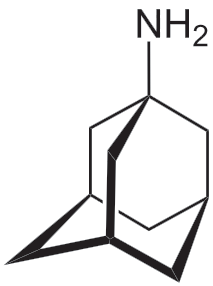
\includegraphics[width=0.25\textwidth]{figures/Amantadina.png}
 \caption{Estuctura química de la Amantadina}
 \label{fig:exemplo}
\end{figure}	

	\section{Docking molecular en interacción con proteínas}
	\label{sec:trab_relacionados}
	
El docking molecular o acoplamiento molecular, es un método bioinformático que permite descubrir y calcular la posición de interacción entre un ligando y un blanco proteico con una representación 3D. Para realizar un problema de acoplamiento molecular se necesita utilizar adecuadamente algoritmos metaheurísticos ya que es un problema de optimización que requiere de varios ajustes y conocimiento de las variables, coordenadas de traslación y movimiento de torsión de la molécula o proteína. La acción farmacológica se produce con la formación de un  complejo  entre  el  fármaco  y  su  receptor  biológico, la cual se  puede optimizar  conociendo  las  estructuras  del  fármaco  y  del  receptor. Así mismo, mediante el  estudio  de dicha interacción entre fármaco y receptor se busca el poder conseguir un compuesto que con la mínima concentración  se forme el   complejo  con  su  receptor  y así generar una respuesta (Font, 2017). 

Por lo tanto, actualmente es una práctica recomendable para conocer la interacción de la amantadina con diferentes aminoácidos en una proteína para bloquear el canal de los protones e interrumpir el ingreso del virus a la célula, especialmente del SARS-Cov-2 (López, García, García, Nebro y Aldana, 2016).  

	
	\section{Metodología}
	\label{sec:metodologia}
	
Para la realización del docking se utilizó el programa AutoDockTools-1.5.6 y AutoDock Vina, la proteína E del SARS-Cov-2, la Amantadina como ligando (DB00915) y los aminoácidos ASN15, LEU18 y LEU19 (Huey, Morris y Forli, 2012) 

Antes de formatear la proteína con AutoDock, se deben resolver varios problemas como incluir átomos faltantes, roturas de cadenas, ubicaciones alternativas y eliminar las aguas cristalográficas. Se inició con subir la proteína al programa y representarla en cintas (figura 2). 


 \begin{figure}[!ht]
 \centering
 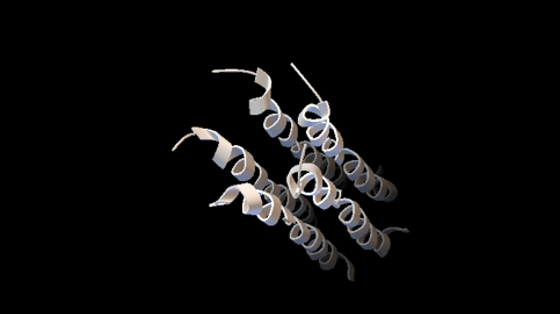
\includegraphics[width=0.70\textwidth]{figures/Ecintas.png}
 \caption{Proteína E}
 \label{fig:exemplo}
\end{figure}
	
	
Después se integró la amantadina (DB00915) como archivo de ligando formateado para AutoDock, ya que debía estar en formato .pdb y contener los tipos de átomos admitidos por AutoDock así como los registros adicionales que especificaran enlaces rotativos (figura 3). 


\begin{figure}[!ht]
 \centering
 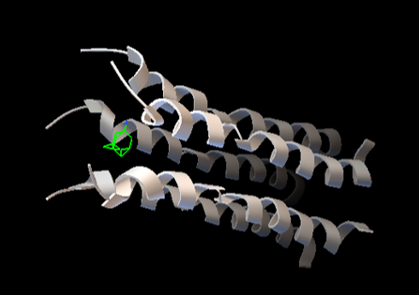
\includegraphics[width=0.70\textwidth]{figures/Eyligando.png}
 \caption{Amantadina (DB00915)}
 \label{fig:exemplo}
\end{figure}
	
	
Se prosigió con la preparación de la macromolécula. Mediante el programa se comprobó que la molécula tenía cargas y se agregaron los hidrógenos. A continuación se configuró el espacio de búsqueda con Grid Box para establecer la ubicación y la extensión del área 3D que se buscó durante el experimento. En este espacio de búsqueda se definió el centro x, y, z, así como el número de puntos en cada dimensión y el espacio entre puntos (figura 4). 
	
	
\begin{figure}[!ht]
 \centering
 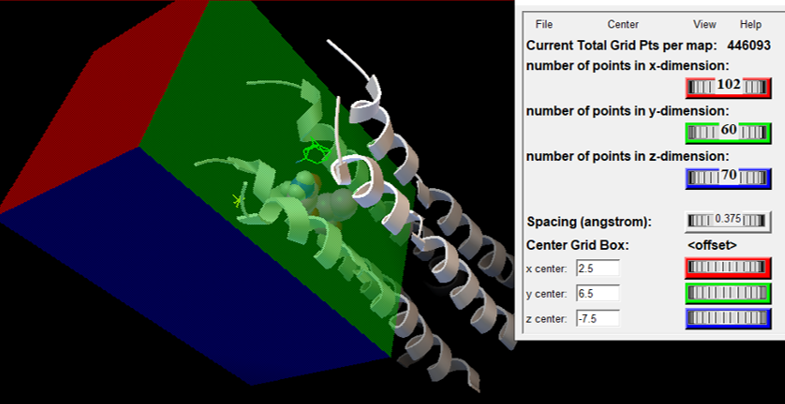
\includegraphics[width=0.70\textwidth]{figures/grid.png}
 \caption{Ubicación y extensión del área 3D}
 \label{fig:exemplo}
\end{figure}
	
	
AutoDock no usa el receptor directamente, utiliza un conjunto de "mapas" precalculados producidos por AutoGrid por lo que el conjunto de mapas debe incluir un mapa para cada tipo de átomo en el ligando de amantadina más dos extras: un mapa "d" para la desolvatación y "e" para la electrostática. 
AutoGrid registra la energía de interacción de un átomo de sonda de un elemento específico en cada punto en una cuadrícula 3D alrededor del receptor rígido en el archivo de mapa de cuadrícula correspondiente. De acuerdo con lo anterior, durante el cálculo de AutoDock, la energía de la configuración del ligando se evaluó con los valores de los mapas de la cuadrícula.

Para la Preparación del archivo de parámetros de AutoDock4 se hizo un acoplamiento corto con 250000 evaluaciones por correr y después se inició el AutoDock4 con AutoDock Vina con el archivo vina.exe. 

En la computadora utilizó un CPU de 8, y una semilla aleatoria (random seed) de 200540960 (figura 5). Por lo que si se quisiera obtener de nuevo este resultado tendría que tomarse en cuenta este mismo parámetro. 


	\begin{figure}[!ht]
 \centering
 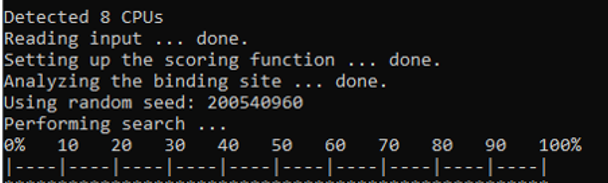
\includegraphics[width=0.70\textwidth]{figures/semilla.png}
 \caption{Semilla Aleatoria del Docking}
 \label{fig:exemplo}
\end{figure}


Posteriormente se obtuvo la energía de afinidad en kcla/mol, de las cuales todas fueron negativas, así como la desviación cuadrática media entre las moléculas y la primera, es decir, qué tanto se parecen a la primera (figura 6). 



	\begin{figure}[!ht]
 \centering
 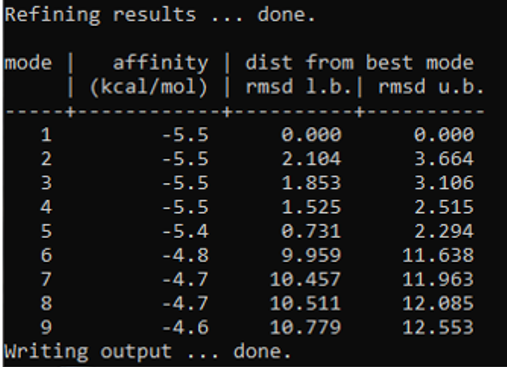
\includegraphics[width=0.70\textwidth]{figures/afinidad.png}
 \caption{Energía de afinidad y desviación cuadrática}
 \label{fig:exemplo}
\end{figure}


Para el resultado de AutoDock Vina se utilizó una sola molécula con múltiples conformaciones para mejor análisis, de los cuales se obtuvieron 9 conformaciones. La energía de afinidad principal fue de -5.5 (figura 7).  


	\begin{figure}[!ht]
 \centering
 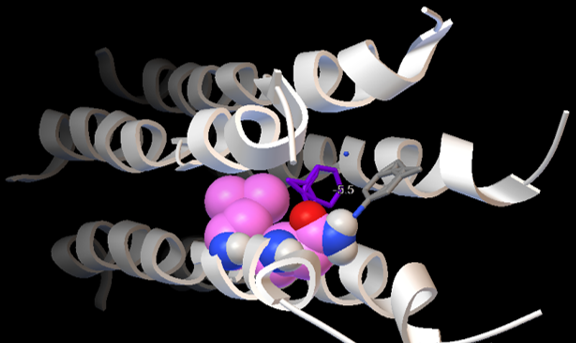
\includegraphics[width=0.70\textwidth]{figures/conformaciones.png}
 \caption{Conformación: Energía de afinidad principal}
 \label{fig:exemplo}
\end{figure}

Por último se realizó el Docking mostrando las interacciones. El ligando se mostró en formas de esferas semi sólidas y los aminoácidos de interacción con el ligando se representaron en jaulas, los átomos con los que interactúa y se siguió mostrando la energía de afinidad (figura 8).  También se muestran todos los residuos en la proteína para ubicar el sitio de interacción y unión (figura 9). 

\begin{figure}[!ht]
 \centering
 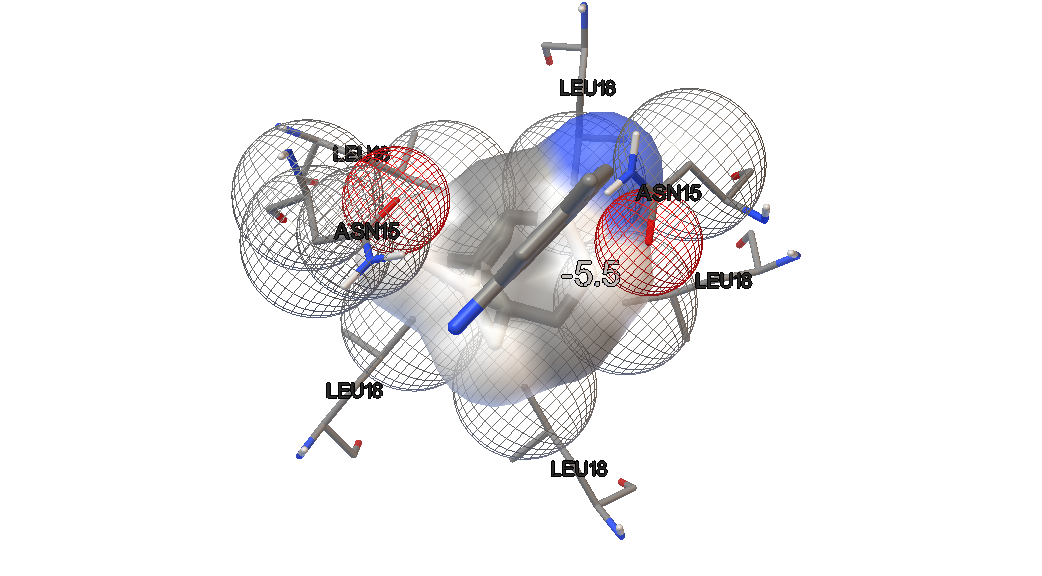
\includegraphics[width=0.90\textwidth]{figures/Aminoacido y ligando.png}
 \caption{Docking con las interacciones}
 \label{fig:exemplo}
\end{figure}


\begin{figure}[!ht]
 \centering
 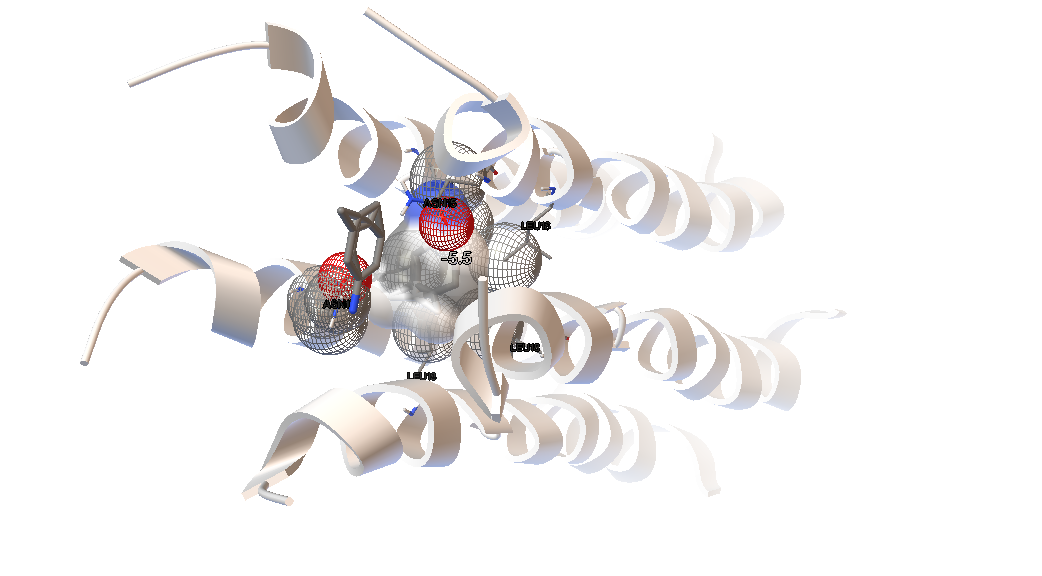
\includegraphics[width=0.90\textwidth]{figures/Interaccion.png}
 \caption{Residuos en la proteína con el sitio de interacción}
 \label{fig:exemplo}
\end{figure}


\section{Conclusiones}
\label{sec:conclusao}
	

El docking molecular es un método que ayuda a conocer la unión más estable, específica y favorable entre un ligando y su blanco para contar con su actividad biológica y saber si es un ligando o fármaco efectivo, por lo tanto, es muy importante en el descubrimiento y desarrollo de nuevos y potenciales fármacos (Ballón y Grados, 2019). Aranda, Hernández, Herrera y Rojas (2020) han propuesto un modelo describiendo a la amantadina como ligando que entra en el canal que se forma por la proteína E del virus para romper los puentes de hidrógeno formados con el agua como lo hace en la influenza A. Por lo que puede recomendarse a la amantadina como inhibidor de la conductancia del canal E en bicapas lipídicas reconstituidas y administrarse cuando se presentan los primeros síntomas de la enfermedad por COVID-19 y así atenuar los efectos del virus. 

Realizar esta actividad permitió conocer los mecanismos del docking molecular, sus herramientas y la interacción de los biomarcadores necesarios para la interacción entre una proteína con su ligando y con los aminoácidos requeridos. Se tuvo que encontrar la forma de realizarlo con diferentes fuentes al igual que el reporte térnico en latex. 


	
\section{Referencias}
\label{chap:Referencias}
1. Aranda, G., Hernández, M., Herrera, D. y Rojas, F. (2020). Amantadine as a drug to mitigate the effects of COVID-19. Medical Hypotheses. 140: 1-3. doi: 10.1016/j.mehy.2020.109755 

2. Araújo, R., Aranda, J. y Aranda, G. (2020). Amantadine Treatment for People with COVID-19. Archives of Medical Research. doi: 10.1016/j.arcmed.2020.06.009

3. Ballón, W. y Grados, R. (2019). Acomplamiento molecular: criterios prácticos para la selección de ligandos biológicamente activos e identificación de nuevos blancos terapéuticos. Revista Con-Ciencia. 2(7): 55-72. 

4. Cortés, M. (2020). Coronavirus como amenaza a la salud pública. Revista Médica de Chile. 148(1).  doi: 10.4067/S0034-98872020000100124.

5. Font, C. (2017). Modelado molecular como herramienta para el descubrimiento de nuevos fármacos que interaccionan con proteínas. Trabajo de fin de grado. Tomado de: http://147.96.70.122/Web/TFG/TFG/Memoria/CRISTINA%20FONT%20MATE.pdf

6. Huey, R., Morris, G. y Forli, S. (2012). Using AutoDock4 and AutoDock Vina with AutoDockTools: A tutorial. USA: The Scripps Research Institute. 

7. López, E., García, M., García, J., Nebro, A. y Aldana, J. (2016). Estudio de estrategias de archivo en PSO multi-objetivo para el Docking molecular. Salamanca.

8. Salazar, M., Peralta, C. y Pastor, F. (2009). Tratado de Psicofarmacología: Bases y aplicación clínica. Buenos Aires: Médica Panamericana. 

9. Terré, R., Pérez, A., Roig, T., Bernabéu, M., y Ramón, S. (2002). Tratamiento farmacológico con amantadina en pacientes con lesión cerebral. Rehabilitación, 36(1), 13–17. doi: 10.1016/s0048-7120(02)73230-1 


\end{document}
